
\section{Momentum Conservation and Center of Mass\footnote{
1990-93 Dept. of Physics and Astronomy, Dickinson College. Supported by FIPSE
(U.S. Dept. of Ed.) and NSF. Portions of this material may have been modified
locally and may not have been classroom tested at Dickinson College.
}}

Name \rule{2.0in}{0.1pt}\hfill{}Section \rule{1.0in}{0.1pt}\hfill{}Date \rule{1.0in}{0.1pt}

\textbf{Objectives }

To explore the applicability of conservation of momentum to the mutual interactions
among objects that experience no external forces (so that the system of objects
is isolated). You will calculate momentum changes for an isolated system consisting
of two very unequal masses and to observe momentum changes for a system consisting
of two equal masses. 

\textbf{Apparatus}

\begin{itemize}
\item Two Pasco dynamics carts with equal masses (and springs, magnets, and velcro). 
\item A track for the carts. 
\item A video analysis system (\textit{VideoPoint}).
\end{itemize}
\textbf{Overview }

You have now tested Newton's third law under different conditions and it always
seems to hold. The implications of that are profound, because whenever an object
experiences a force, another entity must also be experiencing a force of the
same magnitude. A single force is only half of an interaction. Whenever there
are interactions between two or more objects, it is often possible to draw a
boundary around a system of objects and say there is no net external force on
it. A closed system with no external forces on it is known as an isolated system.
Some examples of isolated systems are shown in the figure below.

As a consequence of Newton's laws, momentum is believed to be conserved in isolated
systems. This means that, no matter how many internal interactions occur, the
total momentum of each of the systems pictured below should remain constant.
When one of the objects gains some momentum another part of the system must
lose the same amount of momentum. If momentum doesn't seem to be conserved then
we believe that there is an outside force acting on the system. Thus, by extending
the boundary of the system to include the source of that force we can save our
Law of Momentum Conservation. The ultimate isolated system is the whole universe.
Most astrophysicists believe that momentum is conserved in the universe!

You will begin this unit by examining a situation in which it appears that momentum
is not conserved and then seeing how the Law of Conservation of Momentum can
hold when the whole isolated system is considered. In the next activity you
will make qualitative observations using two carts of equal mass moving toward
each other at the same speed. You will observe momentum changes for several
types of interactions, including an elastic and inelastic collision and an explosion. 

Next, a new quantity, called the center of mass of a system, will be introduced
as an alternate way to keep track of the momentum associated with a system or
an extended body. In the next unit, you will use this concept to demonstrate
that the Law of Conservation of Momentum holds for both one-dimensional and
two-dimensional interactions in isolated systems. Several other attributes of
the center of mass of a system will be studied.

Examples of isolated systems in which the influence of outside forces is negligible
are shown below.

\vspace{0.3cm}
{\par\centering 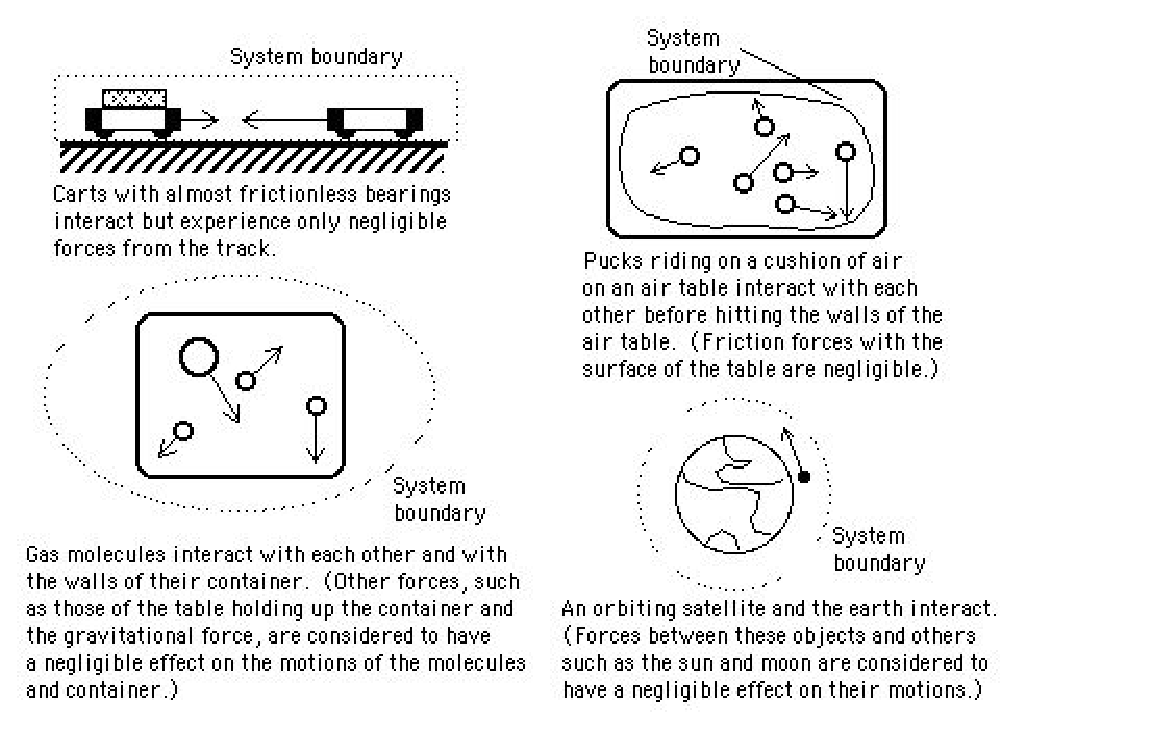
\includegraphics{mom_cons_fig1.eps} \par}
\vspace{0.3cm}

\textbf{When an Irresistible Force Meets an Immovable Object }

Let's assume that a superball and the moon (with an astronaut on it) are the
objects in a closed system. (The pull of the earth doesn't affect the falling
ball, the astronaut, or the moon nearly as much as they affect each other.)
Suppose that the astronaut drops the superball and it falls toward the moon
so that it rebounds at the same speed it had just before it hit. If momentum
is conserved in the interaction between the ball and the moon, can we notice
the moon recoil? 

\textbf{Activity 1: Whapping the Moon with a Superball} 

(a) Suppose a ball of mass 0.20 kg is dropped and falls toward the surface of
the moon so that it hits the ground with a speed of 40 m/s and rebounds with
the same speed. According to the Law of Conservation of Momentum, what is the
velocity of recoil of the moon?

\vspace{0.3cm}
{\par\raggedright 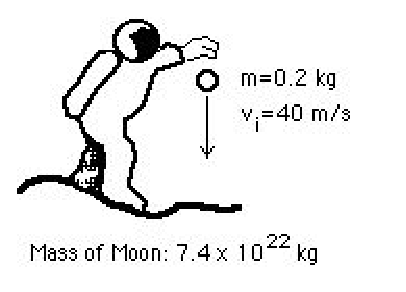
\includegraphics{mom_cons_fig2.eps} \par}
\vspace{0.3cm}

(b) Will the astronaut notice the jerk as the moon recoils from him? Why or
why not?
\vspace{20mm}

(c) Consider the ball and the moon as an interacting system with no other outside
forces. Why might the astronaut (who hasn't taken physics yet!) have the illusion
that momentum isn't conserved in the interaction between the ball and the moon?
\vspace{20mm}

(d) Why might an introductory physics student here on earth have the impression
when throwing a ball against the floor or a wall that momentum isn't conserved?
\vspace{20mm}

\textbf{Collisions with Equal Masses: What Do You Know?} 

Let's use momentum conservation to predict the results of some simple collisions.
The diagrams below show objects of equal mass moving toward each other. If the
track exerts negligible friction on them then the two cart system is isolated.
Assume that the carts have opposite velocities so that \( {{\bf v}_{1i}} 
= - {{\bf v}_{2i}} \). To observe what actually happens, you can
use relatively frictionless carts with springs, magnets, and Velcro.

\textbf{Activity 2: Predictions of the Outcome of Collisions }

(a) Sketch a predicted result of the interaction between two carts that bounce
off each other so their speeds remain unchanged as a result of the collision.
Use arrows to indicate the direction and magnitude of the velocity of each object
after the collision.

\vspace{0.3cm}
{\par\centering 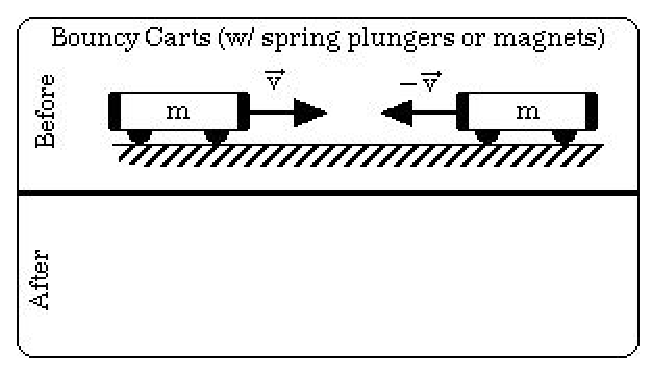
\includegraphics{mom_cons_fig3.eps} \par}
\vspace{0.3cm}

(b) Observe a bouncy collision (also known as an elastic collision) and discuss
whether or not the outcome was what you predicted it to be. If not, draw a new
sketch with arrows indicating the magnitudes and directions of the velocities.
What is the apparent relationship between the final velocities \( {{\bf v}_{1f}} \)
and \( {{\bf v}_{2f}} \)? How do their magnitudes compare to those
of the initial velocities?
\vspace{20mm}

(c) Sketch the predicted result of the interaction between two objects that
stick to other. Use arrows to indicate the direction and magnitude of the velocity
of each object after the collision.

\vspace{0.3cm}
{\par\centering 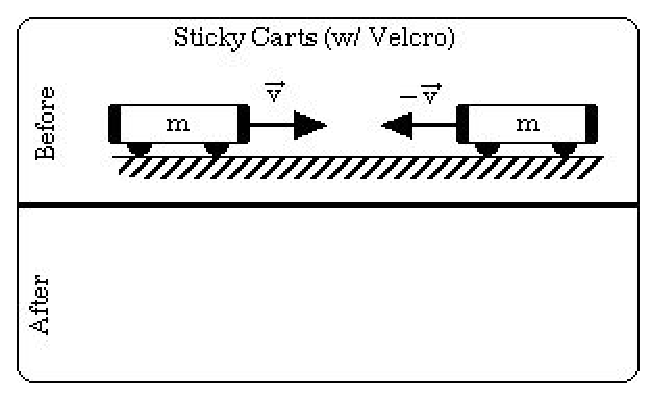
\includegraphics{mom_cons_fig4.eps} \par}
\vspace{0.3cm}

(d) Observe a sticky collision (also known as an inelastic collision) and discuss
whether or not the outcome was what you predicted it to be. If not, draw a new
sketch with arrows indicating the magnitudes and directions of the velocities.
What is the apparent relationship between the final velocities \( {{\bf v}_{1f}} \)
and \( {{\bf v}_{2f}} \)? How do their magnitudes compare to those
of the initial velocities?
\vspace{20mm}

(e) Sketch a predicted result of the interaction between two objects that collide
and then explode. Use arrows to indicate the direction and magnitude of the
velocity of each object after the collision.

\vspace{0.3cm}
{\par\centering 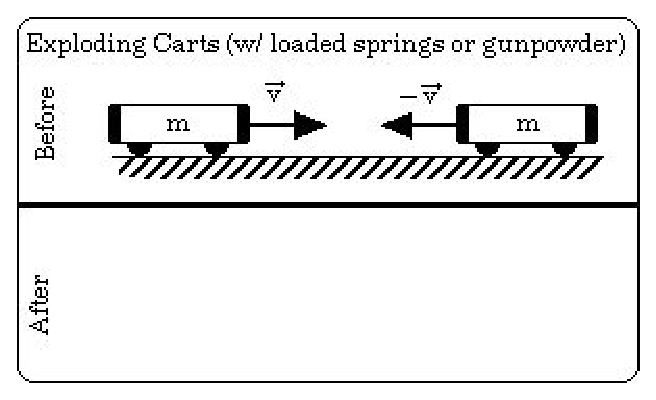
\includegraphics{mom_cons_fig5.eps} \par}
\vspace{0.3cm}

(f) Observe an exploding or ``superelastic'' collision and discuss
whether or not the outcome was what you predicted it to be. If not, draw a new
sketch with arrows indicating the magnitudes and directions of the velocities.
What is the apparent relationship between the final velocities \( {{\bf v}_{1f}} \)
and \( {{\bf v}_{2f}} \)? How do their magnitudes compare to those
of the initial velocities?
\vspace{20mm}

(g) What is the total momentum (i.e., the vector sum of the initial momenta)
before the collision or explosion in all three situations?
\vspace{20mm}

(h) Does momentum appear to be conserved in each case? Is the final total momentum
the same as the initial total momentum of the two cart system?
\vspace{20mm}

\textbf{Defining a Center for a Two Particle System }

What happens to the average position of a system in which two moving carts having
the same mass interact with each other? That is, what happens to 
\(\langle x\rangle = (x_{1} 
+ x_{2} )/2\) as time goes by? What might the motion of the average position
have to do with the total momentum of the system? To study this situation you
will need a video movie-making and analysis system. In making these observations
you'll need to look at the pattern of data points that you place over the frames.
You will not need to create graphs or work with numbers. 

\textbf{Activity 3: Motion of the Average Position} 

(a) Imagine interactions between identical carts moving toward each other at
the same speed as described in Activity 2. Do you expect the average position
of the carts to move before, during, or after the collision or explosion in
each case? Might this have anything to do with the fact that the total momentum
of such a system is zero?
\vspace{20mm}

(b) Let's use video analysis to study a real situation in which the total momentum
of the system is not zero. Do the following: 

\begin{enumerate}
\item Turn the video camera on and center the track in the field of view. The camera
should be about 1 m above the center of the track. Align the track so that it
is parallel to the border of the movie image. Make sure the track is flat by
using the small level available at each station. Place a ruler somewhere in
the field of view where it won't interfere with the collision and parallel to
one side of the field of view. This ruler will be used later to determine the
scale. 
\item Use two carts that have small magnets placed at one end. Make a movie of the
collision of two equal mass carts moving in the same direction with different
speeds. Orient the carts so they collide on the sides that hold the magnets.
See \textbf{Appendix D: Video Analysis} for details on making the movie. When
you save the movie file give it the name \textit{Collision}. 
\end{enumerate}
(c) Determine the average position of both carts during the motion. To do this
task follow the instructions in \textbf{Appendix D: Video Analysis} for creating
and calibrating a data table in VideoPoint. On each frame click once on the
point halfway between the centers of the two carts. When you are finished go
to the \textbf{Edit} menu and highlight \textbf{Leave/Hide Trails}. 

How does the position average appear to move? Might this motion have anything
to do with the fact that the total momentum of the system is directed in one
direction? What is your evidence?
\vspace{20mm}

(d) You should have found that if the momentum of the carts is constant then
the average position moves at a constant rate also. Suppose the masses of the
carts are unequal? How does the average position of the two objects move then?
Lets have a look at a collision between unequal masses. Make and analyze a new
movie as you did before, but add a significant amount of mass to one of the
carts. Once again track the motion of the average position by clicking halfway
between the centers of the two carts. Is the motion of this average position
uniform?
\vspace{20mm}

(e) You should have found the average position of a system of two unequal masses
does not move at a constant velocity. We need to define a new quantity called
the center of mass that is at the center of two equal masses but somewhere else
when one of the masses is larger. Use the video analysis system and your movie
to find a ``center-of-mass location.'' The center of mass is
a location in the isolated system that moves at a constant velocity before,
during, and after the collision. Note: You should be able to make some intelligent
guesses. Describe what you tried and the outcomes in the space below. In the
future you will develop a formal, mathematical definition of the center of mass
and learn about some of its important characteristics. Later, you will apply
the center-of-mass concept to the analysis of momentum conservation in two-dimensional
collisions.

